\documentclass{article}
\usepackage[UTF8]{ctex}
\usepackage{xeCJK}
\usepackage{amsmath}
\usepackage{graphicx}
\usepackage{algorithm}
\usepackage{algorithmic}
\usepackage{listings}
\usepackage{indentfirst}
\usepackage{multirow}
\usepackage[table,xcdraw]{xcolor}
\usepackage{listings}
\usepackage{xcolor}
\usepackage{listings}
\usepackage{placeins}
\usepackage[font={small,stretch=1.25}, justification=raggedright]{caption}
%\usepackage{colortbl}
\usepackage[a4paper,left = 20mm, right = 20mm, top = 12mm, bottom = 12mm]{geometry}
%\captionsetup{font={\fontsize{10.5}{12}\selectfont}} % Set the caption font size to 10.5
% 设置代码样式
\lstset{
    language=Python, % 指定编程语言
    basicstyle=\ttfamily, % 基本字体样式
    keywordstyle=\color{blue}, % 关键字颜色
    commentstyle=\color{green!50!black}, % 注释颜色
    stringstyle=\color{red}, % 字符串颜色
    numbers=left, % 行号位置
    numberstyle=\tiny\color{gray}, % 行号样式
    stepnumber=1, % 行号步长
    numbersep=5pt, % 行号与代码的间距
    backgroundcolor=\color{gray!10}, % 背景颜色
    showspaces=false, % 不显示空格
    showstringspaces=false, % 字符串中不显示空格
    showtabs=false, % 不显示制表符
    tabsize=2 % 制表符宽度
}


\setlength{\parindent}{2em}
% \setCJKmainfont{SimSun}
\renewcommand{\normalsize}{\fontsize{12pt}{14.4pt}\selectfont}



\begin{document}
\begin{titlepage}
    \centering
    \vspace*{\fill}
    {\LARGE\bfseries SIMD NPU设计文档}\\[1.5cm]
    {\Large 郭睿康 22307130115}\\[0.5cm]
    {\Large \today}
    \vspace*{\fill}
\end{titlepage}

\newpage

\section{设计概述}
本次实验设计了一款SIMD的向量处理NPU,旨在通过数据级并行的方式加速矩阵乘加运算。该设计支持8*8规模以下的16位定点矩阵的乘加运算加速,并可以自行配置矩阵的规模进行计算。在指令集架构层面,该设计与Slide中的指令集架构保持一致,在标量指令集的基础上做了向量指令拓展;在硬件架构层面,该设计也与Slide类似,采用了4级流水的RISC结构,同时设置了可以同时读写的标量和向量寄存器堆和存储器,但在实现细节上略有差异,体现在以下几个方面:
\begin{enumerate}
    \item 在MOV指令的实现通路上,添加了一级寄存器以保证所有指令都能够时序对齐,避免了RAR或WAR数据依赖或结构冲突;
    \item 在运算过程中,除了计算阶段,该系统还设计了数据初始化(数据和指令setup)阶段和数据输出阶段,在没有板子的情况下也可以实现高效的仿真验证;
    \item 完善了电路的数据前馈路径,同时将寄存器设置为下降沿写,上升沿读,有效处理了各种指令序列中的数据依赖问题,一定程度上提升了系统的通用性;
    \item 对张量存储器,向量存储器和指令存储器做了统一编址,实现了类似于AXI的简易接口逻辑,用于指令和数据高效的加载和读出,便于系统的仿真验证;
\end{enumerate}
\begin{figure}[!ht]
    \centering
    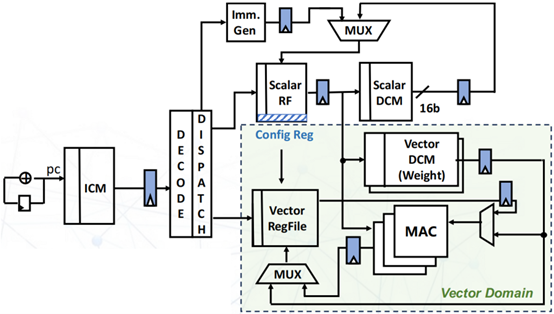
\includegraphics[width=0.8\textwidth]{Arch.png}
    \caption{硬件架构}
\end{figure}

软件架构层面,设计了MATLAB脚本用于生成测试指令序列,该脚本可以根据用户指定的矩阵规模自动生成汇编指令序列,并产生对应的机器码和testbench,可以方便地进行测试和验证。由于整体上架构和Slide中介绍的架构基本相同,下文中只介绍与Slide不同部分的细节。

\subsection{指令集架构}
    该设计的寄存器和总线位宽为16位(数据位宽、地址位宽和指令位宽都是16位),总的可用的地址空间大小为128KB(在该设计中,一个地址就对应16位的数据),然而这么大的空间会耗尽板子上的存储资源,因此只使用其中很小的一部分。统一编址情况如下:
    \begin{figure}[!ht]
        \centering
        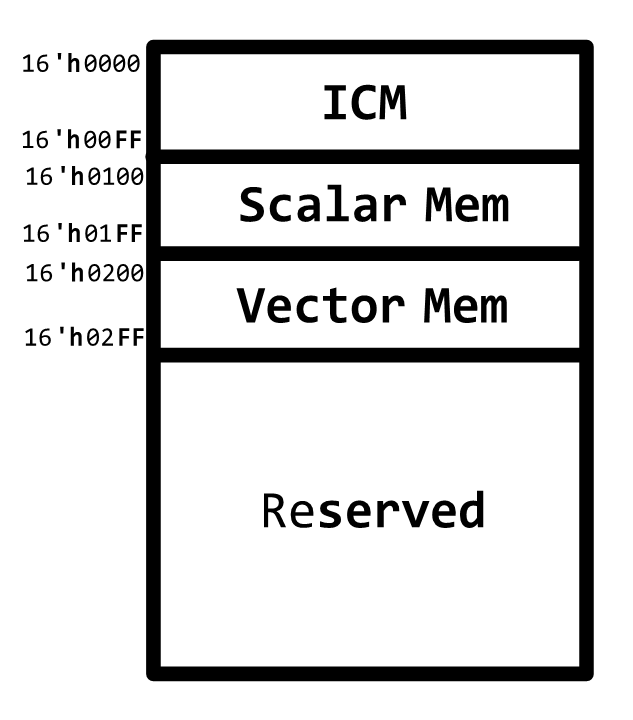
\includegraphics[width = 0.4\textwidth]{Address.png}
        \caption{地址空间分配}
    \end{figure}
    
    该处理机可以接收外部地址,控制器根据地址所在范围将地址自动映射到对应的存储器上进行读写。寄存器方面,总共设置了16个向量寄存器(每个向量寄存器大小为128位,即可以存储8*16位的定点数)和16个标量寄存器(寄存器位宽也为16位)。编号为0的寄存器硬布线到0,编号为15的张量寄存器低8位为vlen,也即当前矩阵规模;高8位为vmask,也即当前矩阵的掩码。其余寄存器均可正常使用。

    指令方面,该处理机支持6种指令,三条标量指令和三条向量指令,指令格式如下所示:
    % Please add the following required packages to your document preamble:
    % \usepackage[table,xcdraw]{xcolor}
    % Beamer presentation requires \usepackage{colortbl} instead of \usepackage[table,xcdraw]{xcolor}
    \begin{table}[!ht]
    \centering
    \caption{指令格式}
    \begin{tabular}{|c|ccc|cccc|ccccccccc|}
    \hline
    \multicolumn{1}{|l|}{}         & \multicolumn{1}{c|}{15} & \multicolumn{1}{c|}{14} & 13 & \multicolumn{1}{c|}{12} & \multicolumn{1}{c|}{11} & \multicolumn{1}{c|}{10} & 9 & \multicolumn{1}{c|}{8} & \multicolumn{1}{c|}{7} & \multicolumn{1}{c|}{6} & \multicolumn{1}{c|}{5} & \multicolumn{1}{c|}{4} & \multicolumn{1}{c|}{3} & \multicolumn{1}{c|}{2} & \multicolumn{1}{c|}{1} & 0                                             \\ \hline
    LOAD                           & \multicolumn{3}{c|}{000}                               & \multicolumn{4}{c|}{rd 4b}                                                      & \multicolumn{4}{c|}{rs1}                                                                          & \multicolumn{5}{c|}{imm5b}                                                                                                                        \\ \hline
    \cellcolor[HTML]{FFFFFF}Store  & \multicolumn{3}{c|}{001}                               & \multicolumn{4}{l|}{\cellcolor[HTML]{000000}}                                   & \multicolumn{4}{c|}{rs1}                                                                          & \multicolumn{4}{c|}{rs2}                                                                          & \multicolumn{1}{l|}{\cellcolor[HTML]{330001}} \\ \hline
    \cellcolor[HTML]{FFFFFF}MOV    & \multicolumn{3}{c|}{010}                               & \multicolumn{4}{c|}{rd 4b}                                                      & \multicolumn{8}{c|}{imm 8b}                                                                                                                                                                           & func 1b                                       \\ \hline
    \cellcolor[HTML]{FFFFFF}Vload  & \multicolumn{3}{c|}{100}                               & \multicolumn{4}{c|}{vrd 4b}                                                     & \multicolumn{4}{c|}{rs1}                                                                          & \multicolumn{5}{c|}{imm5b}                                                                                                                        \\ \hline
    \cellcolor[HTML]{FFFFFF}Vstore & \multicolumn{3}{c|}{101}                               & \multicolumn{4}{l|}{\cellcolor[HTML]{000000}{\color[HTML]{000000} }}            & \multicolumn{4}{c|}{rs1}                                                                          & \multicolumn{4}{c|}{vrs}                                                                          & \multicolumn{1}{l|}{\cellcolor[HTML]{330001}} \\ \hline
    \cellcolor[HTML]{FFFFFF}VMAC-s & \multicolumn{3}{c|}{110}                               & \multicolumn{4}{c|}{vrd 4b}                                                     & \multicolumn{4}{c|}{rs1}                                                                          & \multicolumn{4}{c|}{vrs}                                                                          & func 1b                                       \\ \hline
    \end{tabular}
    \end{table}
    
    指令的功能和Slide中所叙述的完全一致,此处不再一一赘述。值得注意的是,这个指令集的设计并不好,LOAD和Vload中5位的立即数不够8*8规模的矩阵进行寻址。
\subsection{硬件架构}
    硬件架构方面,有如上的四个主要的细节,下面一一阐述。
    \subsubsection{MOV指令的实现通路}
    从原来的架构来看,除了MOV指令,其他所有指令都需要4个周期完成,而MOV只需要3个周期,会提前1个周期写回寄存器。这可能造成不同指令写回阶段的重叠,造成结构冲突,因此在具体实现上,虽然MOV的第三拍是空拍,但还是让它打一拍之后再写回,也就是说要在如下图所示,在立即数写回之前加一个寄存器。

    \begin{figure}[!ht]
        \centering
        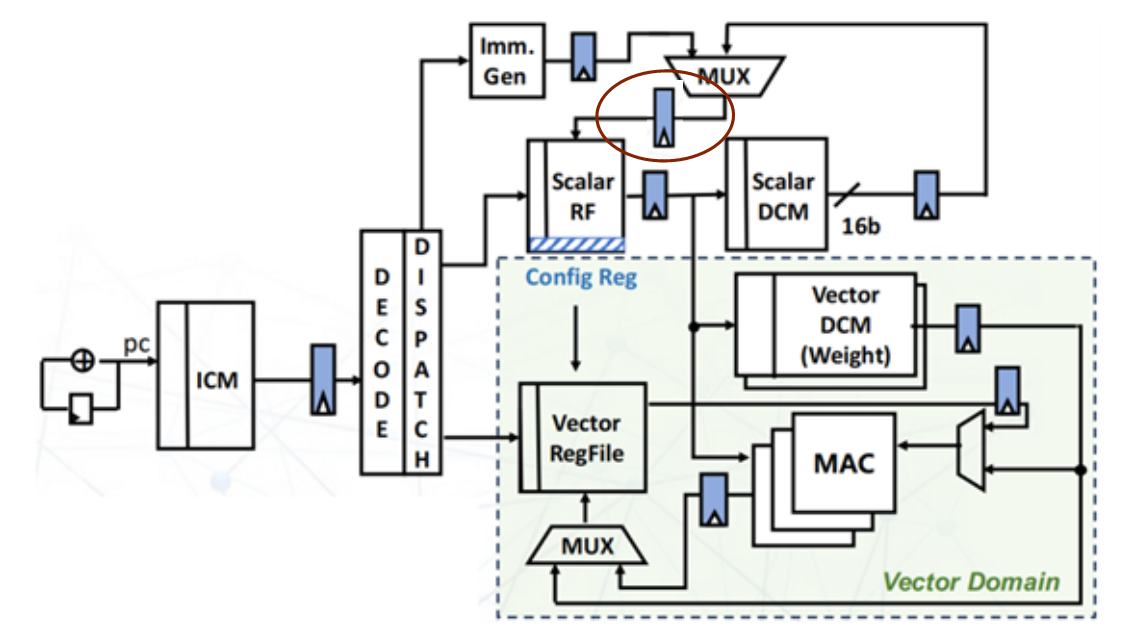
\includegraphics[width = \textwidth]{Arch2.png}
        \caption{改进后的架构}
    \end{figure}

    具体代码细节无需多言。

    \subsubsection{接口逻辑}
    为了简化仿真验证,方便地载入指令数据和读出结果,在处理机的输入和输出侧设计了简易类似于AXI接口逻辑,实现与片外的通信,这里详细介绍数据输入端,输出端是类似的。如下所示,展示了输入端的时序图:
    \begin{figure}[!ht]
        \centering
        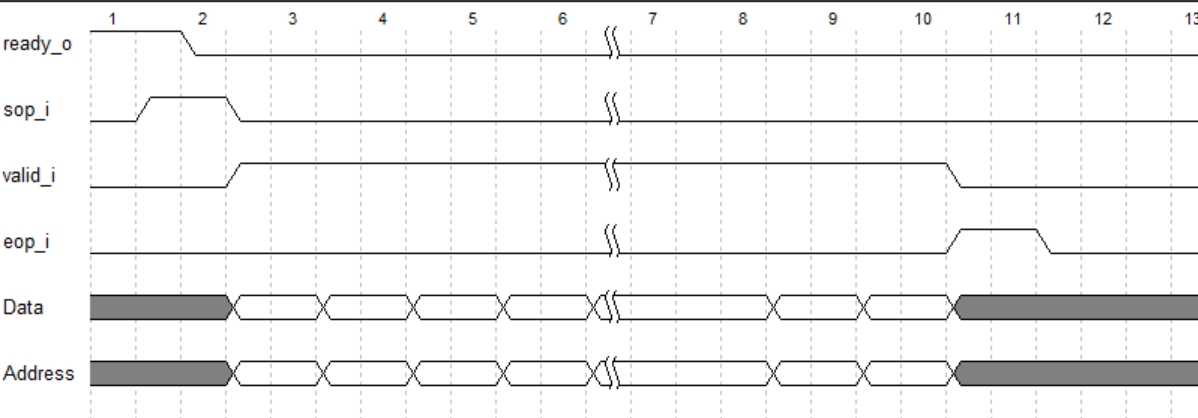
\includegraphics[width = 0.8\textwidth]{Interface_Logic.png}
        \caption{简易AXI接口逻辑}
    \end{figure}
    
    当处理机端准备好接收数据(Ready\_o拉高),外部(CPU)会可以拉高sop\_i表示数据传输开始,下一拍开始传输数据(包括指令)和地址,片上内部控制器将指令映射到正确的物理存储器上,将数据写入存储器或从存储器中读出。地址映射部分代码如下所示:
    \begin{lstlisting}[language=Verilog]
        always @(*)
        begin
            if (state == INIT && valid_i) begin
                if(addr_in_i < SCALAR_BASE) begin
                    wen_init_o = 3'b001;
                end
                else if (addr_in_i < VECTOR_BASE) begin
                    wen_init_o = 3'b010;
                end
                else if (addr_in_i < VECTOR_UPPER) begin
                    wen_init_o = 3'b100;
                end
                else begin
                    wen_init_o = 3'b000;
                end
            end
            else begin
                wen_init_o = 3'b000;
            end
        end
    \end{lstlisting}
    
    wen\_init\_o用于控制初始化阶段向存储器写入数据,是三个存储器的使能信号。

    \subsection{有限状态机设计}
    该处理机的工作流包括五个状态:空闲IDLE、数据和指令初始化INIT、矩阵计算COMP、计算完成DONE、正在写回TRAN。COMP状态完成处理机的核心工作,而另外几个状态则主要用于仿真验证,状态转移的代码如下所示:
    \begin{lstlisting}[language=Verilog]
        always @(*)
        begin
            case (state)
                IDLE: begin
                    if (ready_o && sop_i) begin
                        next_state = INIT;
                    end
                    else begin
                        next_state = IDLE;
                    end
                end

                INIT: begin
                    if (eop_i) begin
                        next_state = COMP;
                    end
                    else begin
                        next_state = INIT;
                    end
                end

                COMP: begin
                    if (complete_o) begin
                        next_state = DONE;
                    end
                    else begin
                        next_state = COMP;
                    end
                end

                DONE: begin
                    if (result_is_OK_o && ready_i)
                        next_state = TRAN;
                    else begin
                        next_state = DONE;
                    end
                end

                TRAN: begin
                    if (trans_complete_o)
                        next_state = IDLE;
                    else
                        next_state = TRAN;        
                end

                default: begin
                    next_state = IDLE;
                end
            endcase
        end
    \end{lstlisting}

    具体细节不赘述,其中的complete\_o,result\_is\_OK\_o,trans\_complete\_o均是由计数器驱动的控制信号,分别用于表征计算完毕、结果已经全部写回向量存储器、结果数据输出完毕。

    \subsection{数据前馈系统}
    原设计中,只考虑了Vload后接VMAC-s指令这一种数据前馈情况,一是没有考虑隔一条的指令之间的数据冒险,二是没有考虑其他很多指令序列可能存在的RAW问题(虽然这样的指令序列不一定会出现)。
    为了解决这两个问题,采用了更加丰富的数据前递策略。将两类寄存器都设置为下降沿写上升沿读,避免了相隔一条指令的两条指令间的RAW问题,在指令译码阶段就能把数据准备好;对于第二个问题,根据指令序列情况设计标志位,对写回数据,写回地址以及MAC单元的操作数进行选择,用传统方法实现数据前递,解决数据还没写回寄存器但已经需要被读的问题。例如如图所示的结构:
    \begin{figure}[!ht]
        \centering
        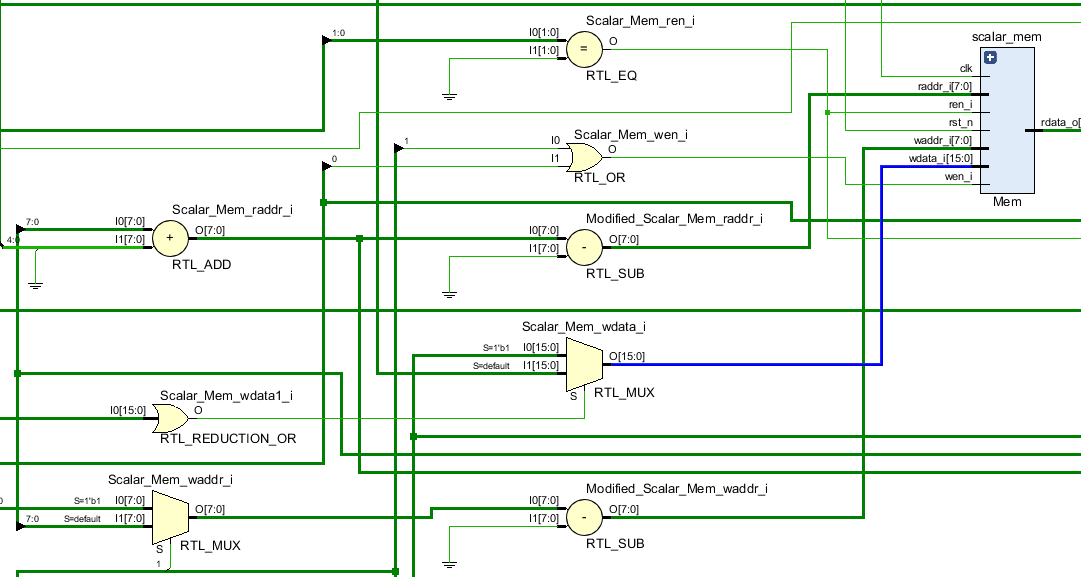
\includegraphics[width = 0.8\textwidth]{Forward.png}
        \caption{数据前递结构示例——标量存储器的地址和数据的数据前递}
    \end{figure}

\subsection{软件架构}
    软件部分直接使用汇编语言编写,并用MATLAB实现了汇编语言的生成和编译脚本,高效完成指令序列的生成和仿真平台的搭建。算法层面采用和Slide中完全一致的策略,将第一个矩阵的元素与第二个矩阵的对应行做向量数乘累加得到结果。略有不同的是,在计算8*8矩阵时,立即数不够用,而又没有实现加法指令,因此要事先产生两个基址,且由于地址是16位的,需要两条MOV指令才能完成基址的加载。报告中贴出了汇编代码片段,供参考。

    \begin{lstlisting}[float,frame=lines]
        MOV r1 02 $1
        MOV r1 00 $0         % Load Base Address
        ...
        MOV r15 8 $0         
        MOV r15 FF $1        % Config Register
        Vload vr1 r1 0 
        VMAC-s vr2 / vr1 $1  % Load Bias
        Load r5 r3 0         % Load Input
        Vload vr1 r2 0       % Load Weight
        VMAC-s vr2 r5 vr1 $0 % MAC Calculation
       ...
        VStore / vr2, r4     % Store Result (wo/ offset)
        MOV r4 02 $1         % Modified result Address
        MOV r4 88 $0         % Modified result Address
    \end{lstlisting}
\subsection{系统setup与验证流程}

系统的setup和验证流程如图所示:
\begin{figure}
    \centering
    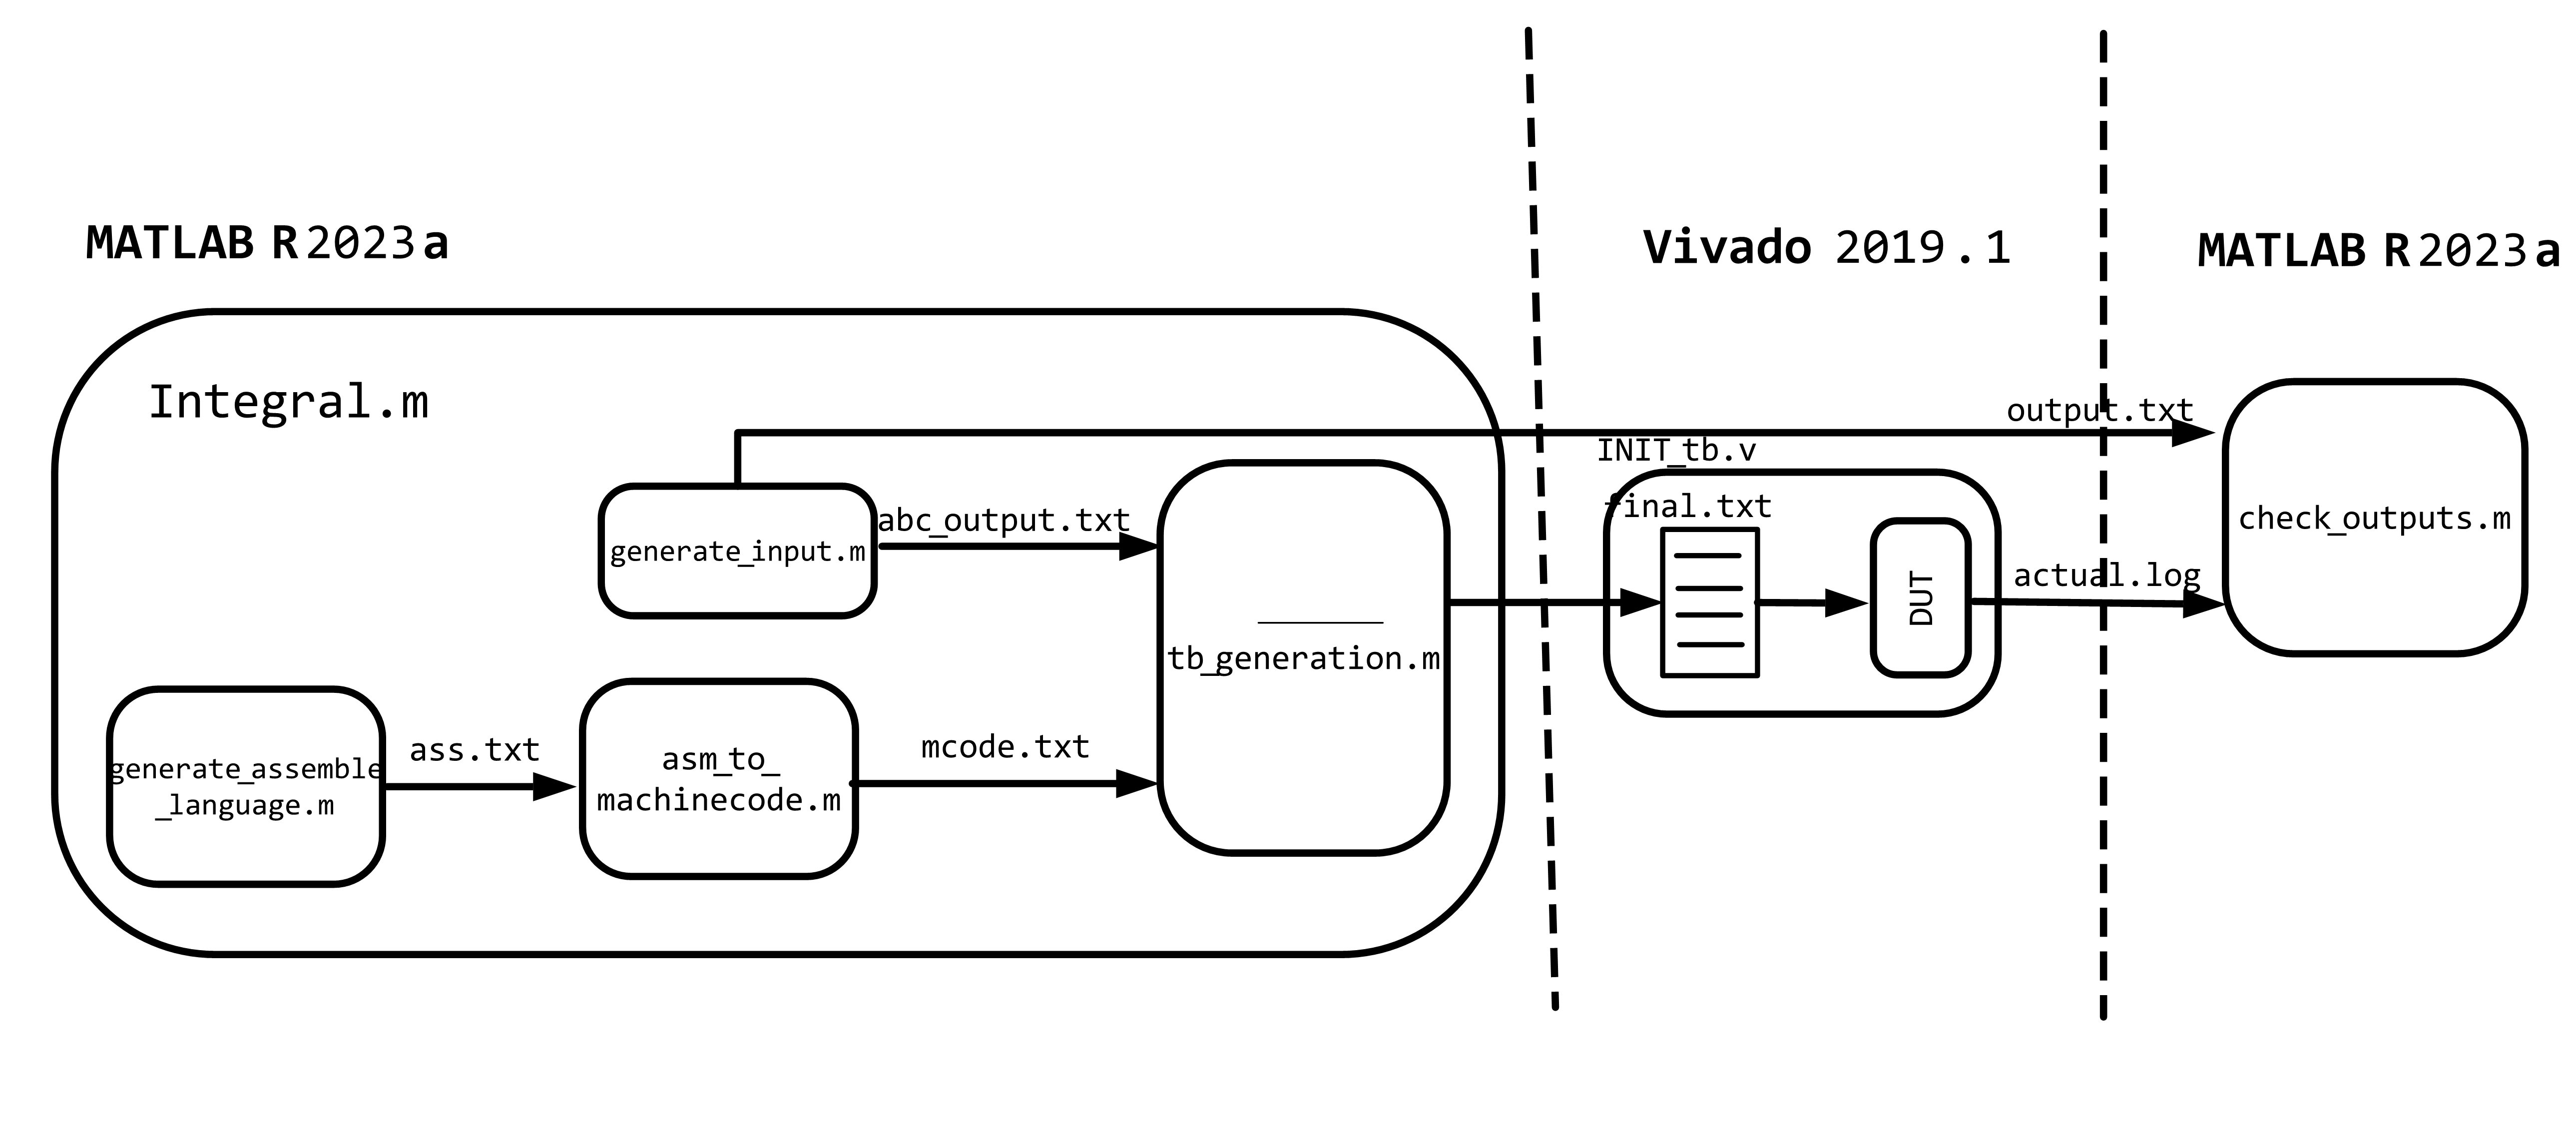
\includegraphics[width = \textwidth]{Flow.png}
    \caption{系统setup与验证流程}
\end{figure}
\newpage
从图中可以看到,利用MATLAB脚本和Verilog语言搭建了联合仿真环境,包括激励生成,仿真运行和结果检查三个部分。其中激励生成和结果检查由MATLAB脚本完成,仿真运行由Verilog语言实现。

在激励生成模块,有四个子模块。
\begin{itemize}
\item Generation\_assemble\_language.m用于生成仅与矩阵规模有关的汇编代码
\item asm\_to\_machinecode.m用于将汇编代码转换为16进制机器码
\item generate\_input.m随机生成测试激励并通过软件计算得到预期结果
\item tb\_generation.m利用机器码和随机生成的测试数据作为testbench数据加载阶段的数据来源,生成testbench的激励文件。
\end{itemize}

将设计好的.v文件在tb中实例化得到仿真结果,最后利用check\_outputs.m检查仿真结果是否正确。具体操作步骤如下:
\begin{enumerate}
    \item 运行``Testbench/Matlab\_TB\_Generation/integral.m''文件夹下的integral.m文件(应确保文件夹下的其他函数对该文件可见),生成testbench的激励文件final.txt,其中包括指令和数据,和若干中间文件。
    \item 将"Testbench/Testbench/INIT\_tb.v"文件中的激励文件地址替换为实际路径(不知道为什么好像一定要用绝对路径),并修改tb中的循环轮数参数,利用该TB在Vivado中进行仿真,得到仿真结果。
    \item 将控制窗口中的仿真结果信息复制出来保存为``Actual.log''文件,在保证能看见前面生成的中间文件result.txt和Actual.log文件的前提下,运行check\_outputs.m脚本,检查仿真结果是否正确。
    \begin{figure}[!ht]
        \centering
        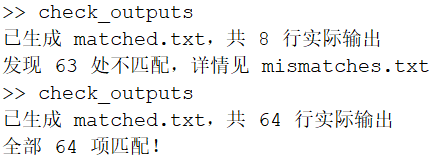
\includegraphics[width = 0.8\textwidth]{仿真结果示例.png}
        \caption{仿真结果示例}
    \end{figure}
\end{enumerate}
\newpage
\section{仿真验证与性能分析}
我们使用xc7z020clg400-1芯片进行综合实现,采用的时钟频率为100MHz。下面的综合实现报告和仿真验证结果
\subsection{资源消耗与性能分析}
DSP和存储资源的消耗如表所示:
\begin{figure}[!ht]
    \centering
    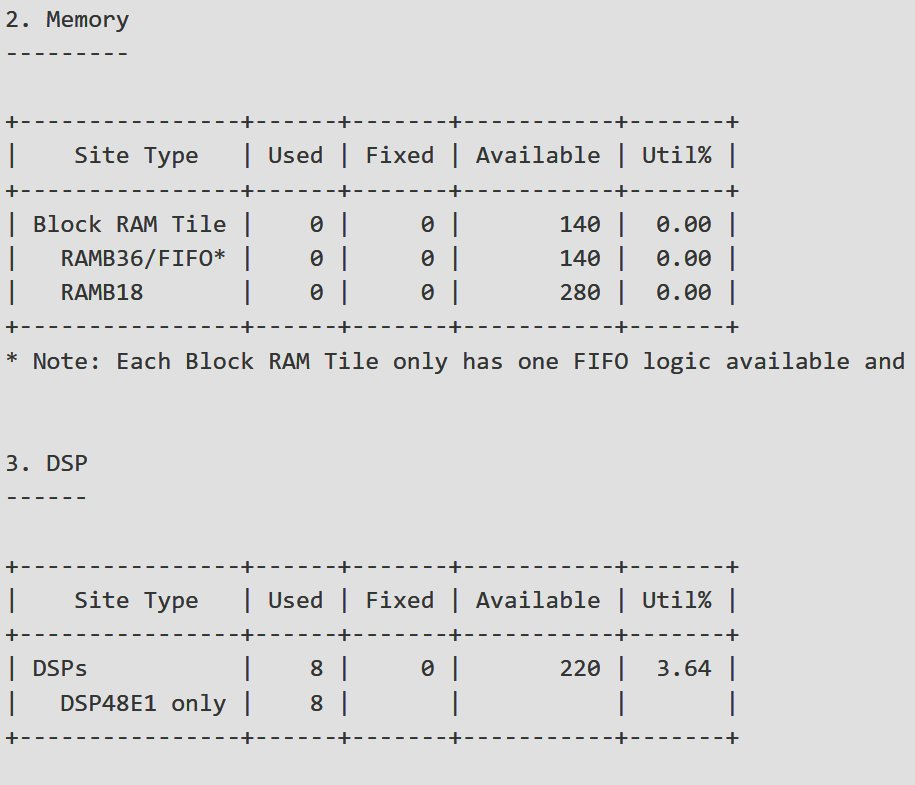
\includegraphics[width = \textwidth]{Utilization.jpg}
    \caption{资源消耗分析}
\end{figure}

更详细的分析可以在log文件夹下的utilization.rpt文件中查看。

时序和功耗的报告如下:
\begin{figure}[!ht]
    \centering
    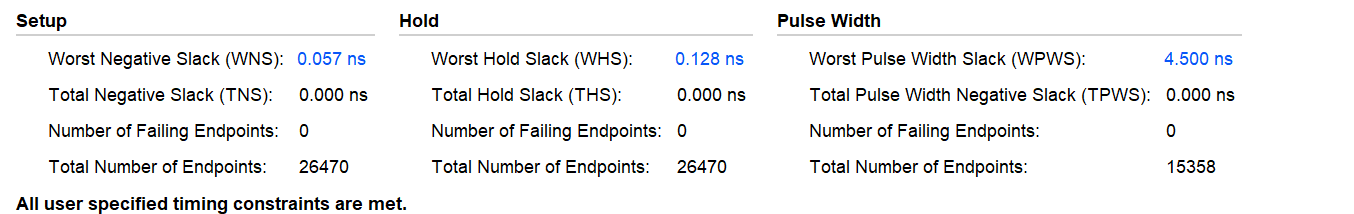
\includegraphics[width = \textwidth]{Timing Report.png}
    \caption{时序报告}
\end{figure}

可以看到时序刚刚好不违例,可用的最大时钟周期大约就是100MHz.

\begin{figure}[!ht]
    \centering
    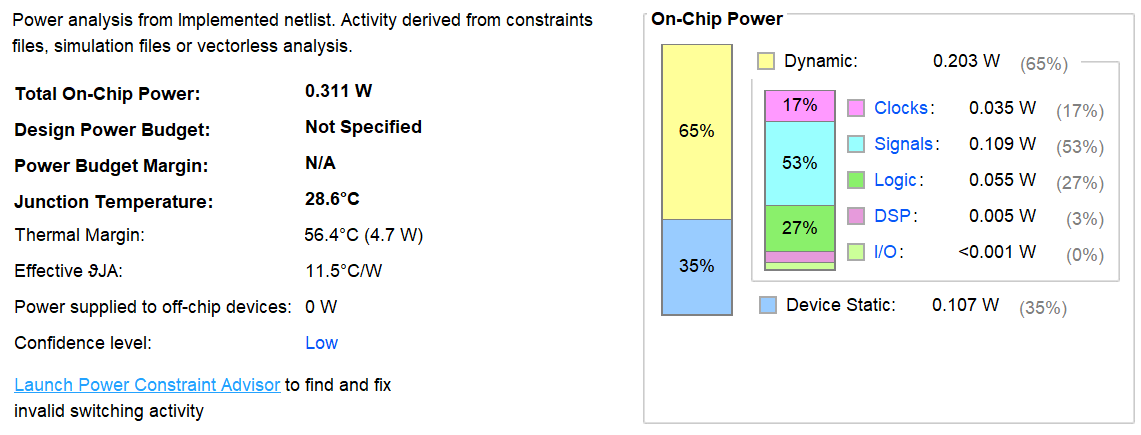
\includegraphics[width = \textwidth]{Power.png}
    \caption{功耗报告}
\end{figure}

下图是宏观的仿真波形:

\begin{figure}[!ht]
    \centering
    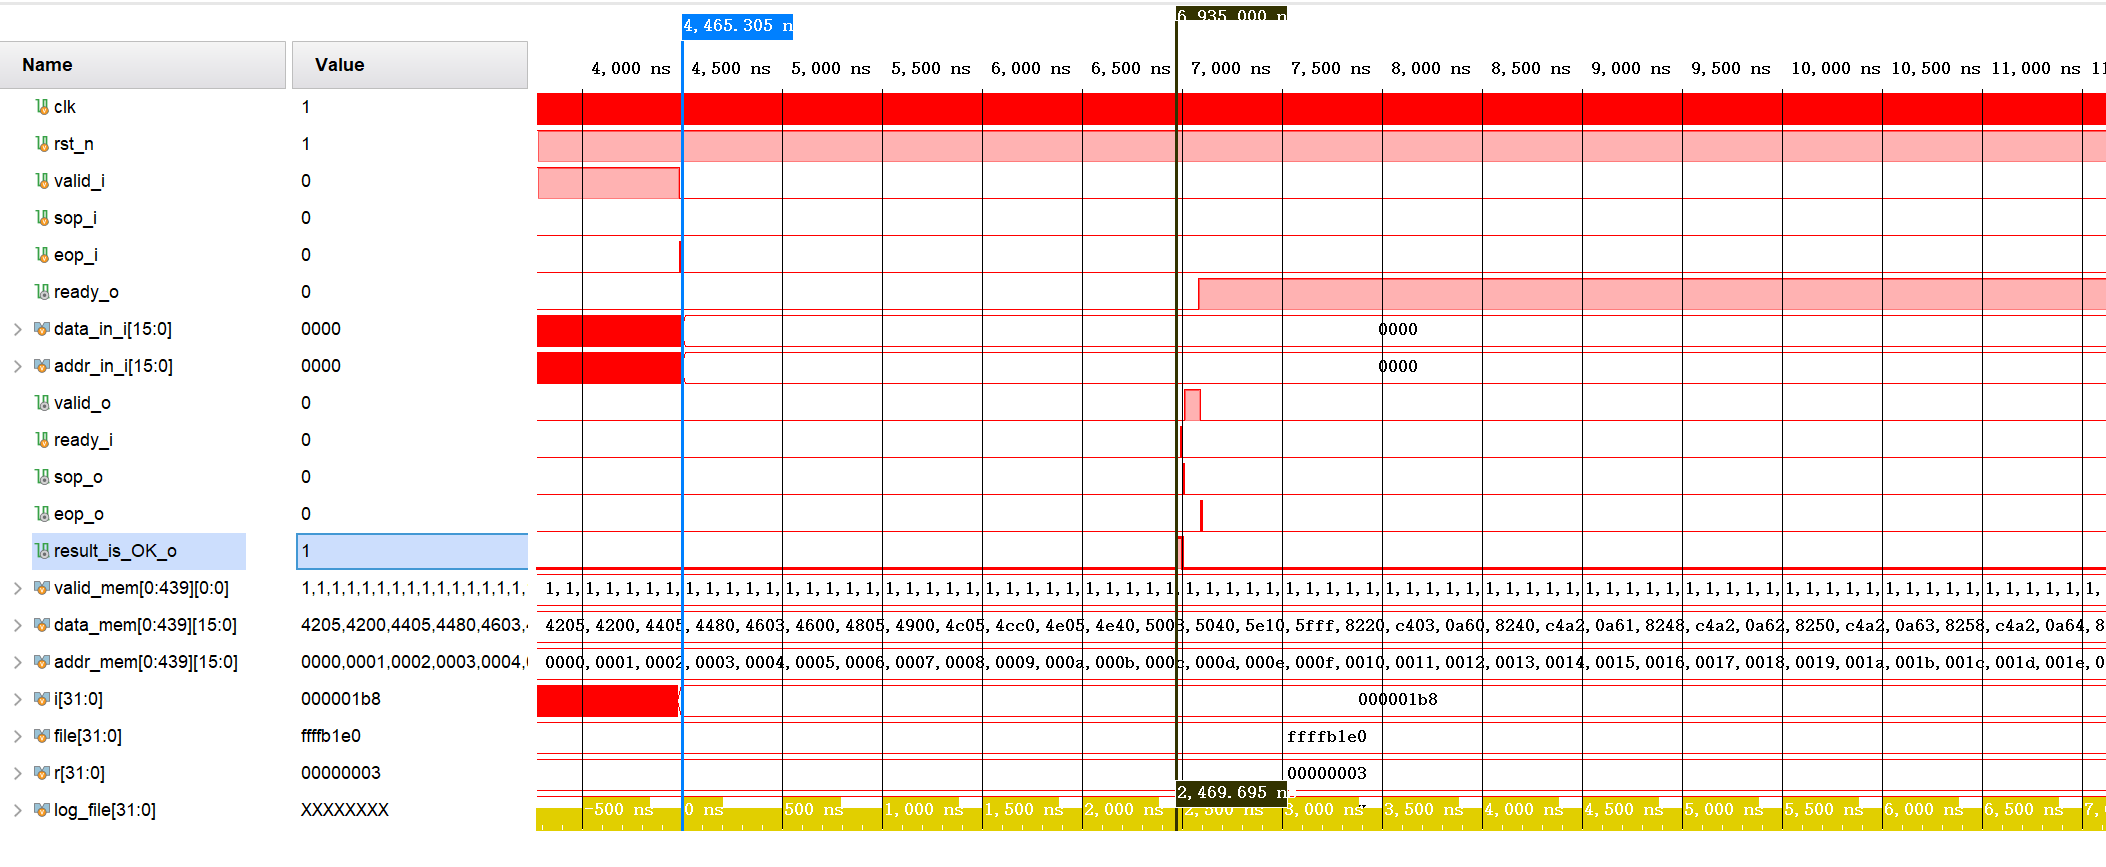
\includegraphics[width = \textwidth]{Sim_1.png}
    \caption{吞吐率计算}
\end{figure}

从波形中不难看出,仿真总共分为三个阶段,中间一个阶段即是计算阶段,对外几乎没有信号输出。给出的波形是矩阵规模为8*8的情形,可以看出从开始计算到运算结果全部写回共耗时2.469$\mu s$,即吞吐率为0.411GFOPS。

\subsection{典型波形与验证结果}
\subsubsection{验证结果}
在给定测试用例下,得到的仿真结果如下图所示:
\begin{figure}[!ht]
    \centering
    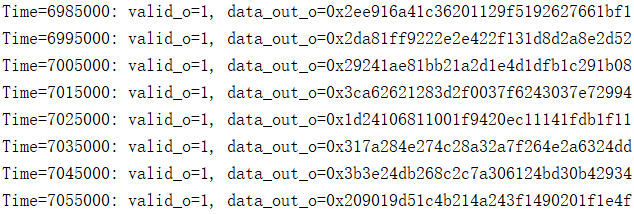
\includegraphics[width = \textwidth]{Sim2.png}
    \caption{仿真结果}
\end{figure}

该结果和软件生成的预期结果完全相同!

\subsubsection{仿真波形}
下面列举了一些比较有代表性的仿真波形。
\begin{figure}[!ht]
    \centering
    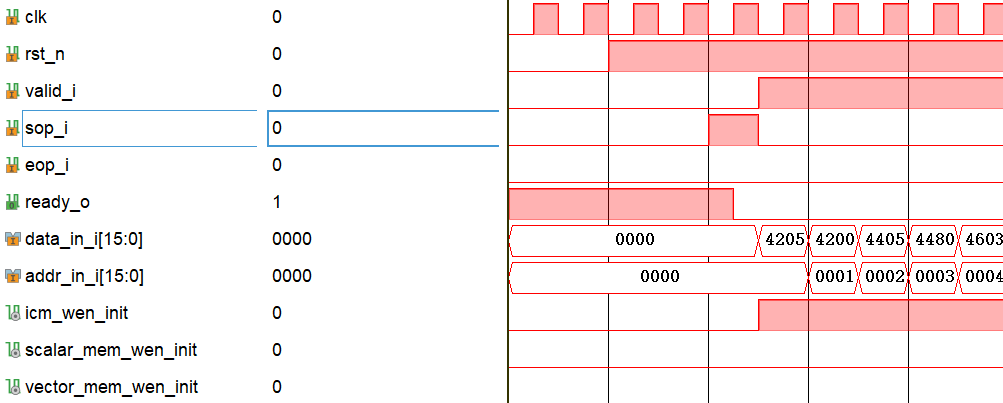
\includegraphics[width = \textwidth]{Input_Interface_Logic.png}
    \caption{输入接口逻辑波形}
\end{figure}

\begin{figure}[!ht]
    \centering
    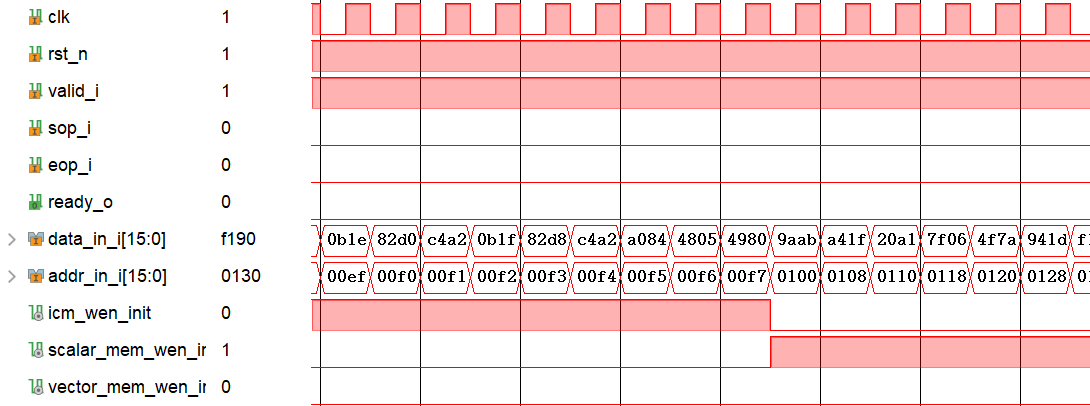
\includegraphics[width = \textwidth]{Addr_Map_Sim.png}
    \caption{地址映射波形}
\end{figure}

\begin{figure}[!ht]
    \centering
    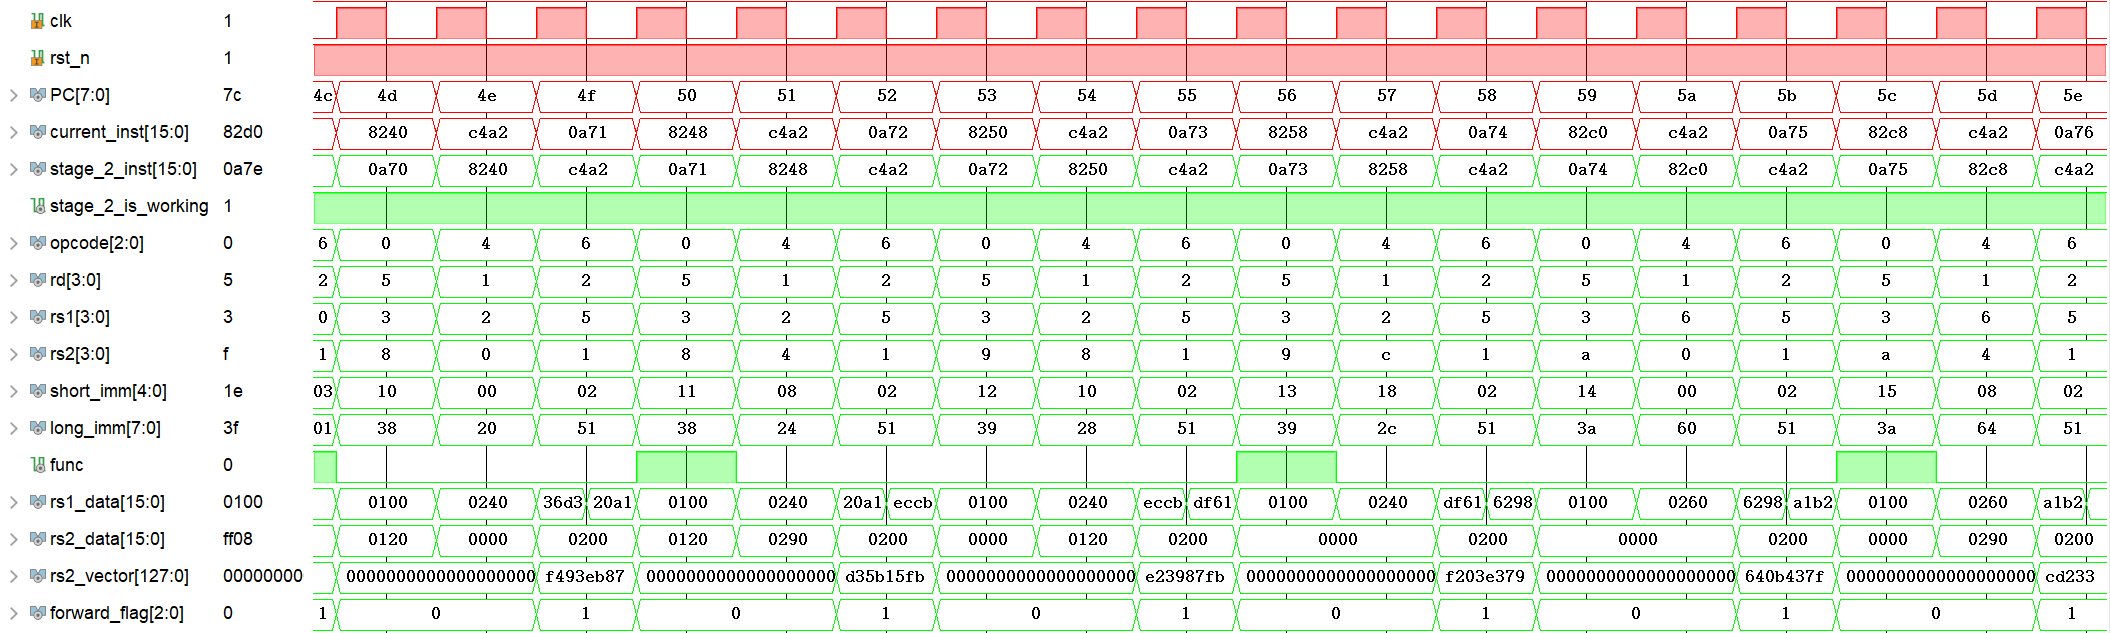
\includegraphics[width = \textwidth]{Pipline1_Sim.png}
    \caption{四级流水线波形1}
\end{figure}

\begin{figure}[!ht]
    \centering
    \includegraphics[width = \textwidth]{Pipline_Sim2.png}
    \caption{四级流水线波形2}
\end{figure}

\begin{figure}[!ht]
    \centering
    \includegraphics[width = \textwidth]{Pipline_Sim3.png}
    \caption{四级流水线波形3}
\end{figure}

\begin{figure}[!ht]
    \centering
    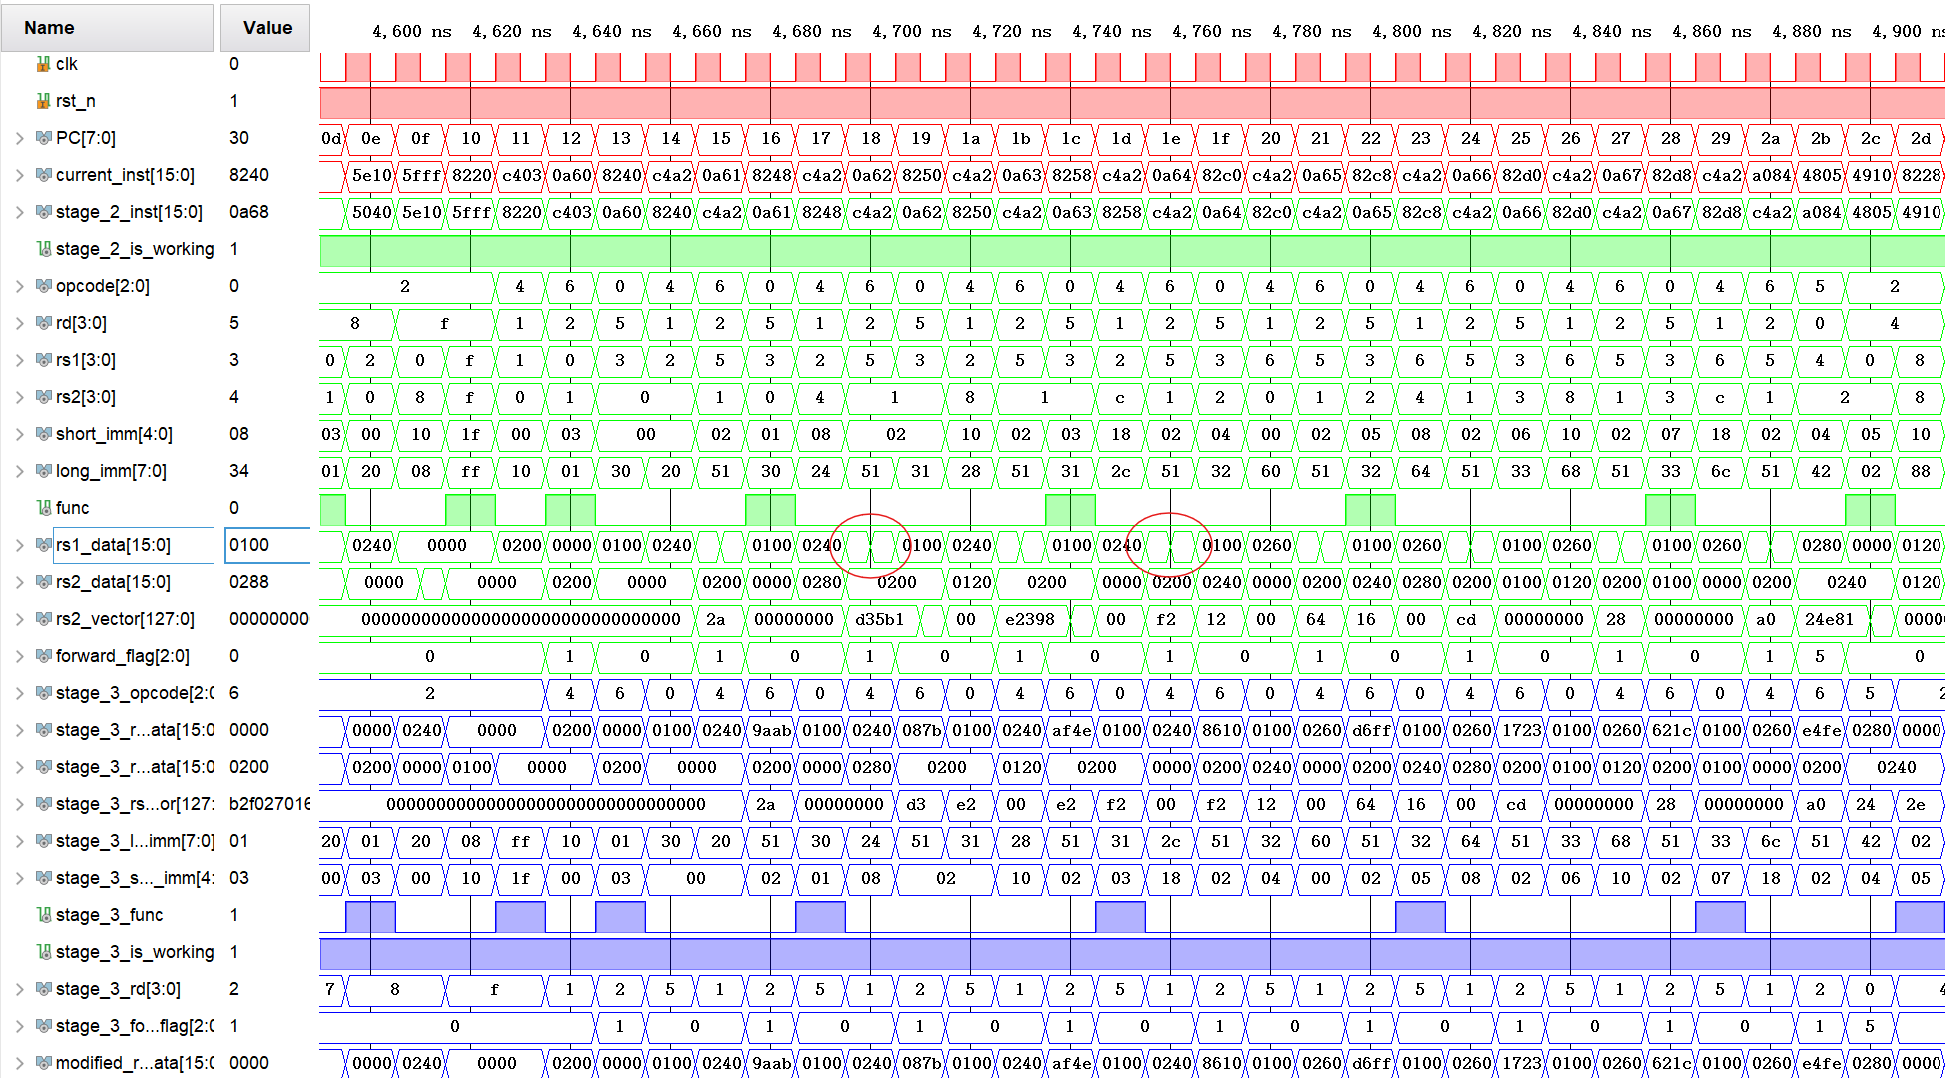
\includegraphics[width = \textwidth]{Forwarding_Sim.png}
    \caption{下降沿写,上升沿读}
\end{figure}

\begin{figure}[!ht]
    \centering
    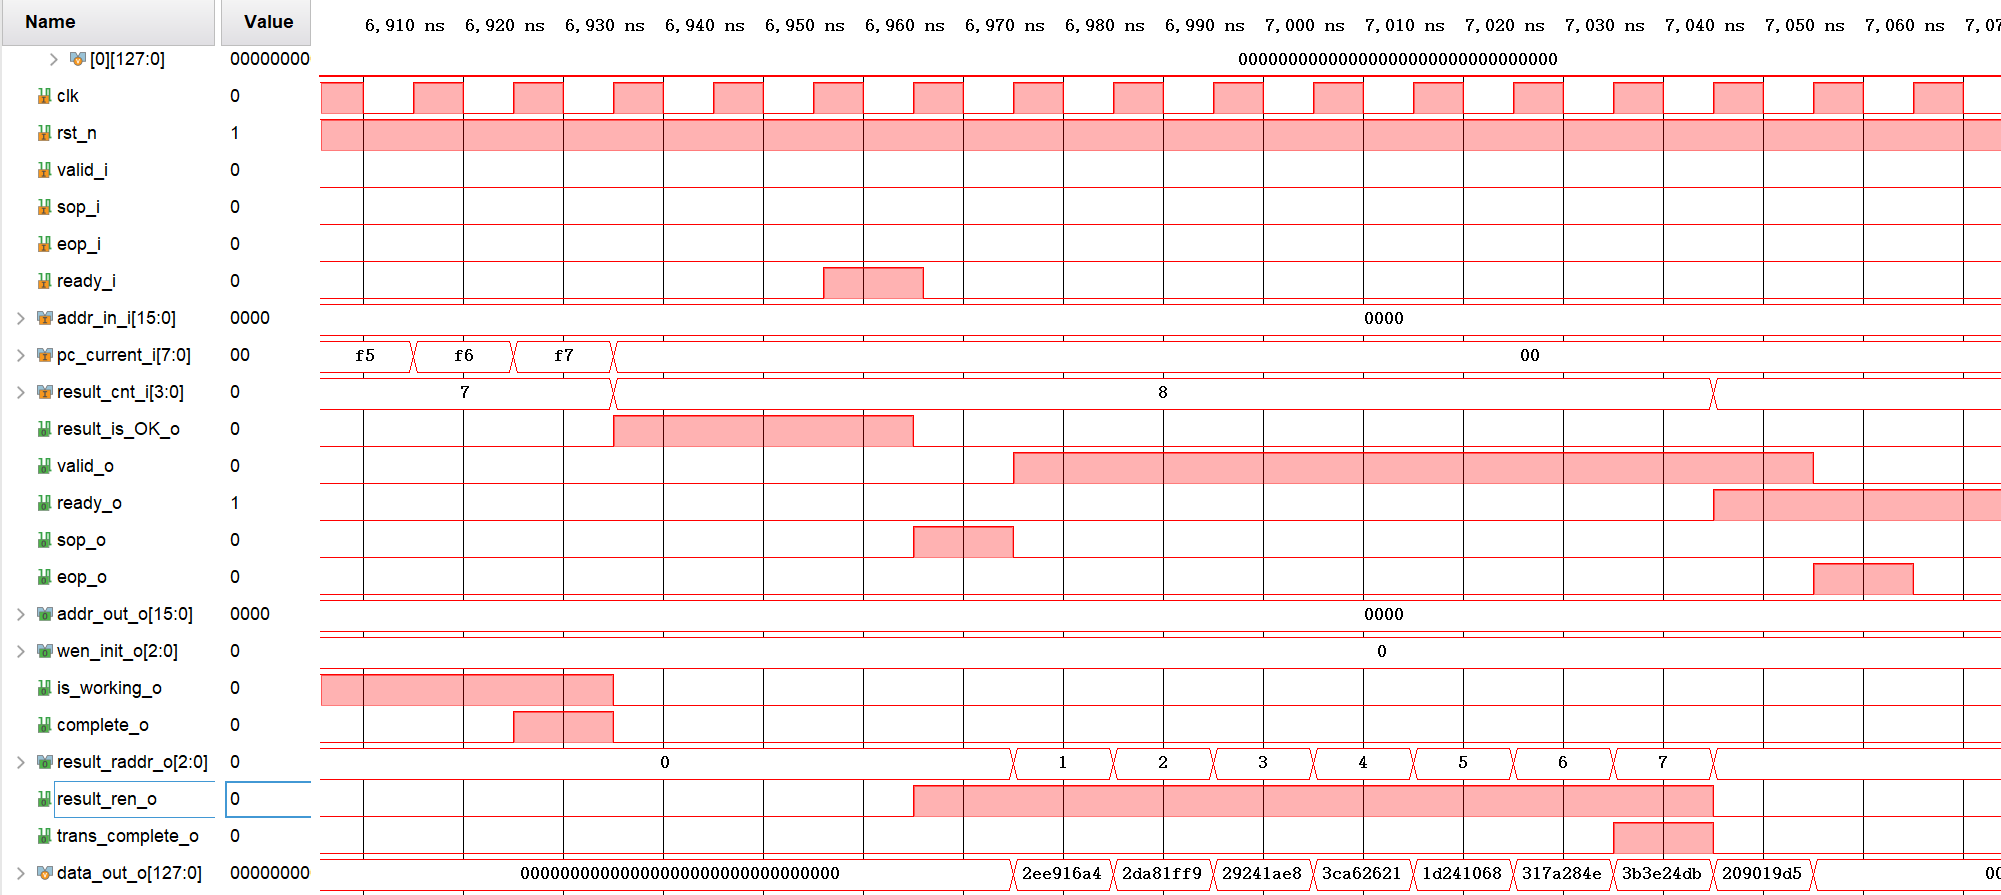
\includegraphics[width = \textwidth]{output_sim.png}
    \caption{输出接口波形}
\end{figure}


\FloatBarrier
\section{优化设计与讨论}
从前面的汇编代码不难看出,这样设计的代码存在很多的冗余,比如大量冗余的、用于加载第二个矩阵行的指令。这些矩阵行显然有复用的潜力却因为所在的向量寄存器被反复覆写而需要被反复加载。从这个角度出发,可以充分利用向量寄存器堆,将16个向量寄存器堆真正当成缓存来用(事实上寄存器堆本来就是全相联的缓存),就可以有效减少指令数量,提高吞吐率。当然由于是软件的优化,不影响硬件结构,硬件的速度和功耗不会发生明显变化(当然若考虑开关活动率和信号跳转方向的差异可能略有区别)。

具体来说,可以将第二个矩阵的若干个矩阵行存在若干个不同的向量寄存器当中,这样只有计算第一行进行``暖身''时需要vload加载,其余行均可复用第一次加载的第二个矩阵,减少指令数量,提高吞吐率。部分代码如下:
\begin{lstlisting}[frame=lines]
        Vload vr1 r1 0
        VMAC-s vr2 / vr1 $1
        Load r5 r3 0
        Vload vr3 r2 0
        VMAC-s vr2 r5 vr3 $0
        Load r5 r3 1
        Vload vr4 r2 8
        VMAC-s vr2 r5 vr4 $0
        Load r5 r3 2
        Vload vr5 r2 16
        VMAC-s vr2 r5 vr5 $0
        Load r5 r3 3
        Vload vr6 r2 24
        VMAC-s vr2 r5 vr6 $0
        Load r5 r3 4
        Vload vr7 r6 0
        VMAC-s vr2 r5 vr7 $0
        Load r5 r3 5
        Vload vr8 r6 8
        VMAC-s vr2 r5 vr8 $0
        Load r5 r3 6
        Vload vr9 r6 16
        VMAC-s vr2 r5 vr9 $0
        Load r5 r3 7
        Vload vr10 r6 24
        VMAC-s vr2 r5 vr10 $0
        VStore / r4 vr2
        MOV r4 02 $1
        MOV r4 88 $0
        ...
    \end{lstlisting}

    仿真得到这个汇编代码的结果是正确的(结果见log文件夹),且比先前的代码少了将近20\%的指令,考虑到这还是访存指令,在实际的处理机中耗时会更长,因此这样的修改是非常有好处的。从仿真结果来看,将汇编代码做此优化后,完成整个矩阵乘加运算的用时减少到了1.911$\mu s$,吞吐率提升至0.569GFOPS,比原先0.411GFOPS的吞吐量增加了将近40\%,这个速度提高是非常显著的。

    \begin{figure}[!ht]
        \centering
        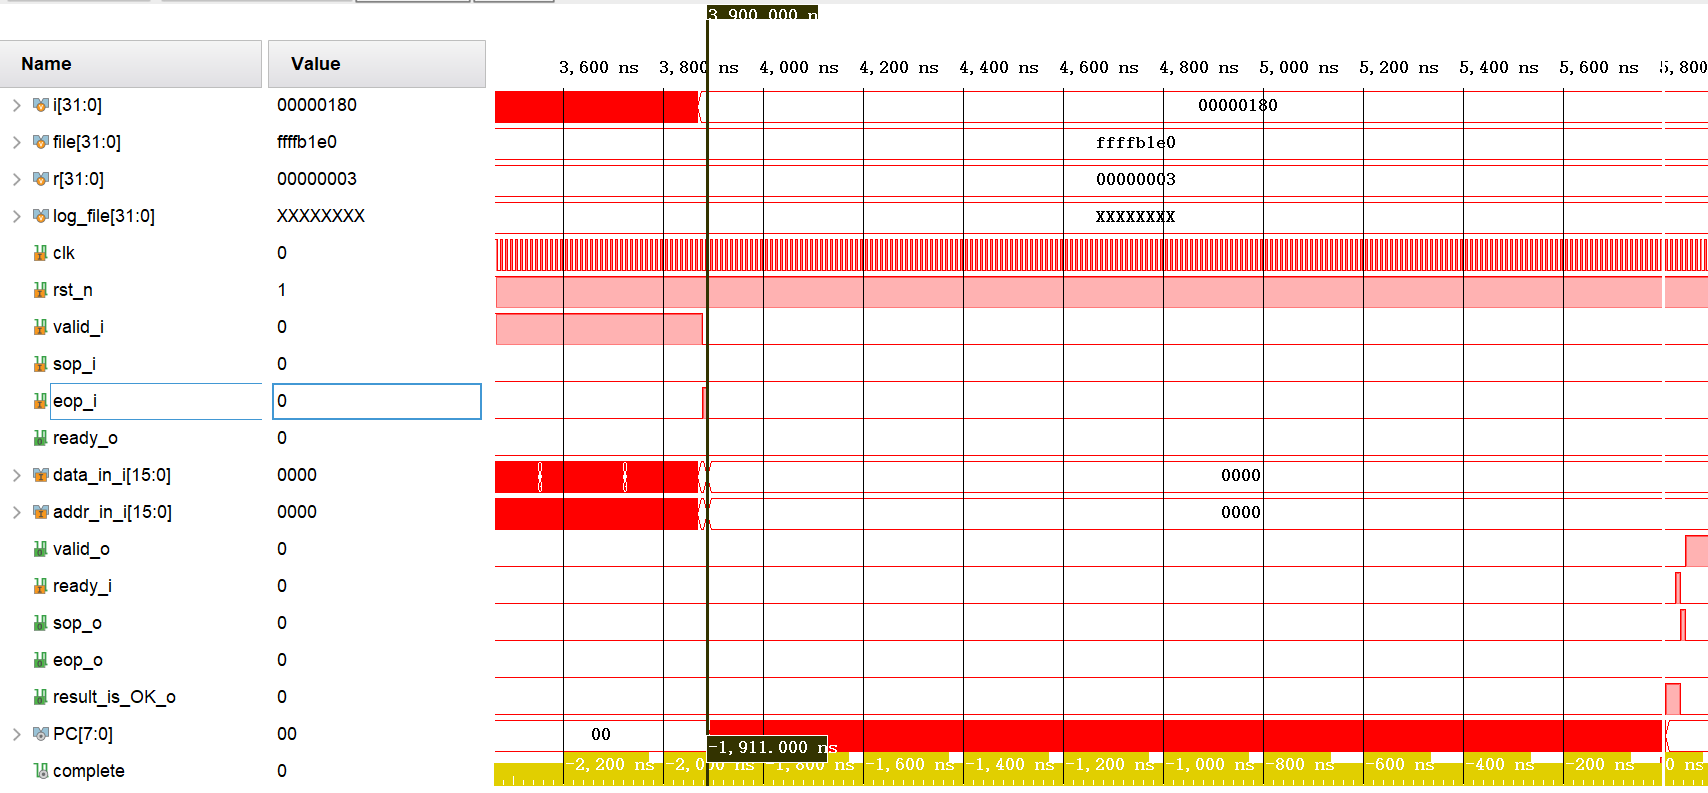
\includegraphics[width = \textwidth]{thp.png}
        \caption{优化后的仿真结果}
    \end{figure}

    这个优化是一个非常浅显的优化,但总体上效果比较明显。除了这种针对软件的优化外,还可以从硬件的角度出发进行优化,如流水化的计算单元等,可以增大同一时刻在运算单元中进行流动的数据量,进而提高吞吐率。但从rtl仿真的层面来看,这种策略的效果不明显,因为存储的带宽基本是够大的。



\section{设计总结}
    本次实验,设计了一款能配置矩阵规模的SIMD矩阵运算加速单元,实现了四级流水线的中的数据级并行,并通过设计输入输出接口逻辑和统一存储空间编址在没有板子的情况下模拟了``CPU+加速器''系统的仿真。通过MATLAB脚本和Verilog语言搭建了联合仿真环境,实现了从汇编代码到硬件的综合实现再到仿真的全过程。在这个过程中,我学习了如何使用Vivado进行硬件加速器的设计,了解了如何搭建仿真环境和编写测试用例,掌握了如何利用MATLAB脚本来实现一个类似于编译器的功能,一定程度上也加深了对算子库和编译器原理的理解。

    总的来说,《智能计算芯片导论》这门课作为一个2分的课,工作量偏大,在上课的过程中感觉没学到什么东西。但是回味起来,好像把之前计体、嵌入式课上没太搞懂的知识都弄清楚了,讲得很宏观但是细节满满,系统性极强,把观念性思想上的东西讲透彻了,在2分课的课时内讲授了3,4分课都讲授不出的知识量。这门课对我来讲是收获颇丰的,结合这学期在FPGA课上学习的内容以及集创赛备赛过程中的学习,我对软硬件的划分,系统级的设计第一次有了非常清晰的认识,虽说这个学期总体过得浑浑噩噩,但是也不能算是完全没学到东西。超级感谢陈老师精心准备的课程,也感谢助教老师们的耐心指导!

\end{document}

